\documentclass[10pt,xcolor={svgnames}]{beamer}
%\usefonttheme[onlymath]{serif}
%%%%% Colors
\usetheme{Dresden}%\usetheme{Madrid}
\colorlet{beamer@blendedblue}{green!55!black}
%%%%%

%%%%% Other 
\beamertemplatenavigationsymbolsempty
\addtobeamertemplate{navigation symbols}{}{%
    \usebeamerfont{footline}%
    \usebeamercolor[fg]{footline}%
    \hspace{1em}%
    \insertframenumber/\inserttotalframenumber
}
%\usepackage{hyperref, url}

\definecolor{pine_green}{HTML}{007935}
%\hypersetup{colorlinks,breaklinks,linkcolor=white,urlcolor=orange,citecolor=black}
\renewcommand\thefootnote{\textcolor{pine_green}{\arabic{footnote}}}

\renewcommand{\i}{\mathnormal{I}}

%\usepackage{cancel}
%\usepackage{ulem}
%\usepackage{multirow}
\usepackage{mathtools}
\usepackage{makecell}
\DeclarePairedDelimiter{\abs}{\lvert}{\rvert}
\renewcommand{\epsilon}{\varepsilon}
\setbeamertemplate{itemize subitem}{\textbullet}
\setbeamertemplate{itemize subsubitem}{$\circ$}

%https://tex.stackexchange.com/questions/289542/auto-resizing-parenthesis-in-math-formulas
% \usepackage{amsmath} for testing
\newcommand*\autoop{\left(}
\newcommand*\autocp{\right)}
\newcommand*\autoob{\left[}
\newcommand*\autocb{\right]}
\AtBeginDocument {%
   \mathcode`( 32768
   \mathcode`) 32768
   \mathcode`[ 32768
   \mathcode`] 32768
   \begingroup
       \lccode`\~`(
       \lowercase{%
   \endgroup
       \let~\autoop
   }\begingroup
       \lccode`\~`)
       \lowercase{%
   \endgroup
       \let~\autocp
   }\begingroup
       \lccode`\~`[
       \lowercase{%
   \endgroup
       \let~\autoob
   }\begingroup
       \lccode`\~`]
       \lowercase{%
   \endgroup
       \let~\autocb
   }}

\delimiterfactor 1001

\makeatletter
% for amsmath "compatibility" (not sophisticated)
% \usepackage{amsmath}
\AtBeginDocument {%
          \def\resetMathstrut@{%
           \setbox\z@\hbox{\the\textfont\symoperators\char40}%
           \ht\Mathstrutbox@\ht\z@ \dp\Mathstrutbox@\dp\z@}%
}%
\makeatother
%%%%%

%%%%% Greying out/invidible Slides
%\setbeamercovered{invisible}
%\setbeamercovered{%
%  again covered={\opaqueness<1->{15}}}
  
%%%%%







%%%%% Footnotes and captions
%\usepackage[utf8]{inputenc}
\usepackage{caption}
%\usepackage{comment}
\setbeamerfont{footnote}{size=\tiny}
\setbeamerfont{caption}{size=\small}
%\setbeamerfont{normal text}{size=\small}
\setbeamerfont{itemize/enumerate body}{size=\small}
\setbeamerfont{itemize/enumerate subbody}{size=\footnotesize}
%%%%%



%Information to be included in the title page:
\title[Connor Wiegand]{Intro to Economic Analysis: Microeconomics}
\subtitle{EC 201 - Day 7 Slides}
\author[EC 201]{Connor Wiegand}
\institute[]{Department of Economics - University of Oregon}
\date{18 October 2021}


\begin{document}

\frame{\titlepage}

\section*{Introduction}

\begin{frame}{Logistics}
    \begin{itemize}
        \item Official homework 3 due this Saturday at 11:59pm, covering last week's material
        \item Next news assignments posted, due next Wednesday (October 27)
        \item Midterm November 3rd
        \begin{itemize}
            \item Bring non-graphing, non-algebra calculator
        \end{itemize}
    \end{itemize}
\end{frame}

\begin{frame}{Recall}
    \begin{itemize}
        \item The price elasticity of demand is given by
        $$\epsilon_{D}=\left|\frac{\%\Delta Q_{D}}{\%\Delta P}\right|$$
        and is interpreted as the \% in quantity demanded for a good falls when price rises by 1\%
        \item The income elasticity of demand is given by 
        $$\epsilon_{\i}=\frac{\%\Delta Q_{D}}{\%\Delta \i}$$
        and is interpreted as the \% in quantity demanded for a good falls when income rises by 1\%
    \end{itemize}
\end{frame}

\begin{frame}{Recall}
    \begin{itemize}
        \item We define elastic/unit-elastic/inelastic as $\epsilon_{D}$ being above/at/below 1
        \item We define inferior/normal/superior as $\epsilon_{\i}$ being below 0/above 0 and below 1/above 1
        \item We calculate percentage changes using the midpoint formula
        $$\epsilon_{D}=\left|\frac{\%\Delta Q_{D}}{\%\Delta P}\right|=\left|\frac{(Q_{2}-Q_{1})/[(Q_{1}+Q_{2})/2]}{(P_{2}-P_{1})/[(P_{1}+P_{2})/2]}\right|$$
    \end{itemize}
\end{frame}

\section*{CPED}

\begin{frame}{Cross-Price Elasticity of Demand}
    \begin{itemize}[<+->]
        \item The other demand elasticity we will talk about is the \underline{\textbf{Cross-Price}} \underline{\textbf{Elasticity of Demand}} (CPED)\footnote{\vspace{1mm} As an aside, the existence of cross-price elasticity of demand leads some economists to refer to the price elasticity of demand as the ``\textit{Own} price elasticity of demand"}
        \item For this elasticity, we need two goods: $x$ and $y$
        \item Important: The Cross-Price Elasticity of Demand \underline{\textit{for good $x$ with respect to good $y$}} is defined as 
        $$\epsilon_{xy}=\frac{\%\Delta Q_{x}}{\%\Delta P_{y}}$$
        \item The important part here is the order, as it is easy to get confused which good goes on the top versus which one goes on the bottom
        \item Here, $Q_{x}$ is still taken to be the quantity demanded ($Q_{D}$) of $x$, but I have omitted $D$ to avoid clutter\footnote{\vspace{1mm}You can write $Q_{D_{x}}$, if you would like}
    \end{itemize}
\end{frame}

\begin{frame}{Interpretation of CPED}
    \begin{itemize}[<+->]
        \item The textbook defines CPED as the ``measure of how much the quantity demanded of one good responds to a change in the price of another good, computed as the percentage change in quantity demanded of the first good divided by the percentage change in price of the second good"
        \item In a similar style to the other elasticities, if the cross price elasticity of $x$ with respect to $y$ is given by $\epsilon_{xy}$, then we say that if the price of $y$ rises by 1\%, then the quantity demanded for good $x$ changes by $\epsilon_{xy}\%$ 
    \end{itemize}
\end{frame}

\begin{frame}{Purpose of CPED}
    \begin{itemize}[<+->]
        \item The reason we use CPED is to determine whether two goods are complements or substitutes -- let's think about which sign should be which
        \item When $y$ is a substitute for $x$, we expect that an increase in the price of $y$ leads to a(n)...
        \begin{itemize}
            \item increase in the quantity demanded of $x$, meaning $\epsilon_{xy}$ should be...
            \item positive
        \end{itemize}
        \item Likewise, when $y$ is a complement to $x$, we expect that an increase in the price of $y$ leads to a decrease in the quantity demanded of $x$, so $\epsilon_{xy}$ should be negative
    \end{itemize}
\end{frame}

\begin{frame}{CPED, by numbers}
Goods $x$ and $y$ are said to be...
    \begin{itemize}[<+->]
        \item \textit{complements} if $\epsilon_{xy}<0$
        \begin{itemize}
            \item \textit{perfect complements} if $\epsilon_{xy}=-\infty$
            \begin{itemize}
                \item Close example: left and right shoes
            \end{itemize}
        \end{itemize}
        \item \textit{unrelated} if $\epsilon_{xy}=0$
        \item \textit{substitutes} if $\epsilon_{xy}<0$
        \begin{itemize}
            \item \textit{perfect substitutes} if $\epsilon_{xy}=\infty$
            \begin{itemize}
                \item Close example: any goods which are similar enough for you to only care about price: two brands of butter, triple sec, cheap coffee, etc.
            \end{itemize}
        \end{itemize}
    \end{itemize}
\end{frame}

\begin{frame}{An Obscure Aside}
    \begin{itemize}[<+->]
        \item Q: Is the CPED symmetric? I.e., does $\epsilon_{xy}=\epsilon_{yx}$?
        \begin{itemize}
            \item An increase in the price of a gaming console means less video games will get consumed, but does that mean that if video games get more expensive, people will reduce their console consumption by a similar amount?
            \item Alternatively, do you think that a change in the price of sprite will affect the demand for coke in the exact same way that a change in the price of coke will affect the demand for sprite? 
        \end{itemize}
        \item A: Probably not, so an interesting fact of CPEDs is that they are not necessarily symmetric
        \item Any interesting examples you can think of?
    \end{itemize}
\end{frame}

\begin{frame}{Exercise 1}
    \begin{itemize}[<+->]
        \item Suppose that when berries rise in price by 16\%, the demand for cream falls from 20 oz to 18 oz
        \item However, when the price of cream rises by 16\%, the demand for berries falls from 30 oz to 20 oz
        \item Calculate $\epsilon_{bc}$ and $\epsilon_{cb}$. Are berries and cream substitutes, complements, or neither?
    \end{itemize}
\end{frame}

\begin{frame}{Solution 1}
    \begin{itemize}[<+->]
        \item \begin{align*}
            \epsilon_{cb}=\frac{[(18-20)/19]\cdot 100}{16}=-\frac{10.53}{16}=-0.658
        \end{align*}
        \item \begin{align*}
            \epsilon_{bc}=\frac{[(20-30)/25]\cdot 100}{16}=-\frac{40}{16}=-2.5
        \end{align*}
        \item The goods are complements, note that they are asymmetric
    \end{itemize}
\end{frame}

\section*{Elasticity and Ceteris Paribus}

\begin{frame}{Recall: Ceteris Paribus}
    \begin{itemize}[<+->]
        \item Recall my ceteris paribus example:
        \begin{itemize}
            \item You want to find the impact that time of year has on gas prices, so you decide to compare gas price averages across different months: Jan-Jan, Feb-Feb, etc. Your sample years are 2020 and 2021
        \end{itemize}
        \item Picking 2020 and 2021 will not give you an accurate measure of how time of year impacts gas, because COVID had such large impacts on everything
        \item In the same spirit, what would happen if the price of good $x$ changed between the two data points you were using to calculate income elasticity?
    \end{itemize}
\end{frame}

\begin{frame}{Elasticity and Ceteris Paribus (cont.)}
    \begin{figure}
        \centering
        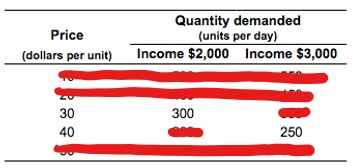
\includegraphics[width=7cm]{cet_par example 1.jpg}
        \caption*{I have two points with different $Q_{D}$ and $\i$. Can you calculate income elasticity using these two data points? What about PED?}
    \end{figure}
\end{frame}

\begin{frame}{Elasticity and Ceteris Paribus (cont.)}
    \begin{itemize}[<+->]
        \item Suppose you land a job at Amazon, and are tasked with calculating the price elasticity of demand for soda
        \item After a year of market research, you find the price elasticity of demand for Dr. Pepper 0.82
        \item However, you neglected to notice that Pibb Xtra (Mr. Pibb) was running huge sales all year. Is that a big deal?
        \item A: \textbf{yes}. There are problems with all of these. Without keeping everything else constant, we have no way to separate out the effects from different price and income movements
        \begin{itemize}
            \item You can't know that a 1\% increase in price decreases demand for Dr. Pepper by 0.82\%, because, for all you know, most of the demand decrease you saw came from Mr. Pibb sales
            \item Likewise, the decrease in the demand for mushrooms could very well have been from the price increase (we actually know it is, because we found mushrooms to be a normal good earlier). Moreover, the income change increase could have stunted this observation about price elasticity
        \end{itemize}
    \end{itemize}
\end{frame}

\begin{frame}{Exercise 2}
    \begin{itemize}[<+->]
        \item Consider the following table for beer and wine
        \begin{table}[]
            \centering
            \begin{tabular}{c|c|c|c|c}
            \textbf{Year} & \thead{\textbf{$P_{w}$/bottle}\\(\$)}
            & \thead{\textbf{$P_{b}$/can}\\(\$)} & \thead{\textbf{Income}\\(\$)} & \thead{\textbf{$Q_{D}$ of Wine}\\(cases/year)}  \\
            \hline
            1 & 1.40 & 1.20 & 25k & 20k \\
            2 & 1.40 & 1.20 & 25k & 20k \\
            3 & 1.00 & 1.00 & 25k & 15k \\
            4 & 1.00 & 1.40 & 25k & 25k \\
            5 & 1.00 & 1.40 & 30k & 15k \\
            6 & 1.40 & 1.40 & 30k & 5k
            \end{tabular}
        \end{table}
        \item Compute $\epsilon_{D_{w}}$, $\epsilon_{\i_{w}}$, and $\epsilon_{wb}$
    \end{itemize}
\end{frame}

\begin{frame}{Solution 2}
    \begin{itemize}[<+->]
        \item $1\to 2$: 
        \begin{itemize}
            \item Nothing changes, can't do anything, so we can't do anything
        \end{itemize} 
        \item $2\to3$:
        \begin{itemize}
            \item Prices change simultaneously, so we do not have all else equal: can't compute any elasticities
        \end{itemize} 
        \item $3\to4$ 
        \begin{itemize}
            \item Only the price of beer changes\footnote{Here and throughout, When I mean ``only", I mean between prices and income, only one changes}, so we can calculate the cross-price elasticity of demand for wine with respect to beer:
            $$\epsilon_{wb}=\frac{(15k-5k)/10k}{(1.4-1)/1.2}=3$$
            \item Therefore, beer and wine are substitutes
        \end{itemize}
    \end{itemize}
\end{frame}

\begin{frame}{Solution 2 (cont.)}
    \begin{itemize}[<+->]
        \item $3\to4$ 
        \begin{itemize}
            \item Only the price of beer changes, so we can calculate the cross-price elasticity of demand for wine with respect to beer:
            $$\epsilon_{wb}=\frac{(25k-15k)/20k}{(1.4-1)/1.2}=1.5$$
            \item Therefore, beer and wine are substitutes
        \end{itemize}
        \item $4\to5$ 
        \begin{itemize}
            \item Only income changes, so we can calculate income elasticity of demand:
            $$\epsilon_{\i}=\frac{(15k-25k)/20k}{(35k-25k)/30k}=-1.5$$
            \item Therefore, wine is an inferior good
        \end{itemize}
        \item $5\to6$ 
        \begin{itemize}
            \item Only the price of wine changes, so we can calculate the PED for wine:
            $$\epsilon_{D}=\frac{(15k-5k)/10k}{(1.4-1)/1.2}=3$$
            \item Therefore, demand for wine is elastic
        \end{itemize}
    \end{itemize}
\end{frame}

\begin{frame}{Remark}
    \begin{itemize}[<+->]
        \item Using the same table as above,
        \begin{table}[]
            \centering
            \begin{tabular}{c|c|c|c|c}
            \textbf{Year} & \thead{\textbf{$P_{w}$/bottle}\\(\$)}
            & \thead{\textbf{$P_{b}$/can}\\(\$)} & \thead{\textbf{Income}\\(\$)} & \thead{\textbf{$Q_{D}$ of Wine}\\(cases/year)}  \\
            \hline
            1 & 1.40 & 1.20 & 25k & 20k \\
            2 & 1.40 & 1.20 & 25k & 20k \\
            3 & 1.00 & 1.00 & 25k & 15k \\
            4 & 1.00 & 1.40 & 25k & 25k \\
            5 & 1.00 & 1.40 & 30k & 15k \\
            6 & 1.40 & 1.40 & 30k & 5k
            \end{tabular}
        \end{table}
        \item What about $\epsilon_{D_{b}}$, $\epsilon_{\i_{b}}$, or $\epsilon_{bw}$?
        \begin{itemize}
            \item We can't compute them, not enough info
        \end{itemize}
    \end{itemize}
\end{frame}

\begin{frame}{Takeaway}
    \begin{itemize}[<+->]
        \item To effectively calculate elasticities, you have to have other relevant factors held constant
        \item This is the tough task of many experimental and data-driven economists: finding data and using techniques such that you can isolate meaningful results that you are confident in
    \end{itemize}
\end{frame}

\section*{Elasticity of Supply}

\begin{frame}{Supply Elasticities}
    \begin{itemize}[<+->]
        \item Just like we could measure how sensitive consumers were to changes in price, we can measure how sensitive producers are to changes in price as well
        \item Of course, we could also think to measure other supply elasticities, but we will limit ourselves to only computing the \underline{price} elasticity of supply
        \begin{itemize}
            \item For this reason, I may refer to the price elasticity of supply as just the ``elasticity of supply" 
        \end{itemize}
        \item Note that the elasticity of supply will be very similar to the PED
    \end{itemize}
\end{frame}

\begin{frame}{Price Elasticity of Supply}
    \begin{itemize}[<+->]
        \item The definition of \underline{\textbf{price elasticity of supply}} for a good, $\epsilon_{S}$, is given by 
        $$\epsilon_{S}=\frac{\% \Delta Q_{S}}{\% \Delta P}$$
        \item $\epsilon_{S}$ measures the sensitivity of producers to supply, given changes in price
        \begin{itemize}
            \item Supply of a good is said to be \textit{elastic} if the quantity supplied responds substantially to changes in the price
            \item Supply is said to be inelastic if the quantity supplied responds only slightly to changes in the price
        \end{itemize}
        \item Am I missing absolute values?
        \begin{itemize}
            \item No, because the law of supply says that quantity supplied increases with price, so this object is already positive
        \end{itemize}
    \end{itemize}
\end{frame}

\begin{frame}{PES, by numbers}
    \begin{itemize}[<+->]
        \item Just like PED,
        \item When $\epsilon_{S}<1$, we say that supply is \textit{inelastic}
        \begin{itemize}
            \item This says that producers are relatively insensitive to changes in price
            \item When $\epsilon_{S}=0$, we say that supply is \textit{perfectly inelastic}
        \end{itemize}
        \item When $\epsilon_{S}>1$, we say that supply is \textit{elastic}
        \begin{itemize}
            \item This says that producers are relatively sensitive to changes in price
            \item When $\epsilon_{S}=\infty$, we say that supply is \textit{perfectly elastic}
        \end{itemize}
        \item When $\epsilon_{S}=1$, we say that suply is \textit{unit-elastic}
    \end{itemize}
\end{frame}

\begin{frame}{Determinants of PES}
    \begin{itemize}[<+->]
        \item While multiple things can affect supply elasticity, there are two key determinants
    \end{itemize}
    \begin{enumerate}
        \item Availability of the product or of raw materials:
        \begin{itemize}
            \item If there is a fixed availability of a product, then (reasonable) changes in price are unlikely to affect quantity supplied
            \begin{itemize}
                \item Ex: You would have to increase the price of a Picasso painting significantly to get someone to sell
                \item Ex: Gold is mined at around 2,500-3,000 tons/year. While an increase in price can induce owners and managers to try to work miners harder, it would take a significant price increase in gold to induce the mine owners to build new infrastructure to increase the rate of mining 
            \end{itemize}
        \end{itemize}
        \item Time Horizon:
        \begin{itemize}
            \item Just like demand, supply is price-sensitive in the long run
            \item Suppliers who already have product developed and ready to sell are often willing to make price corrections in the moment, but will likely change their production behavior in the long run
        \end{itemize}
    \end{enumerate}
\end{frame}

\begin{frame}{Determinants of PES}
    \begin{itemize}[<+->]
        \item Other things that may affect the PES include storage capacity, ``convertability" of inputs, complexity of production process, etc. 
        \begin{itemize}
            \item Markets in which sellers have the ability to store large amounts of product are able to be less sensitive to price changes
            \item If your land or factory can be easily converted to producing in another market, you will be more price insensitive -- if the price is too low, you drop out of the market
            \item Related to availability and convertability, producers with straightforward production processes can start, stop, and change their supply levels easily, making them less sensitive to prices
            \begin{itemize}
                \item Conversely, those with large, complicated processes are more price-sensitive 
            \end{itemize}
        \end{itemize}
    \end{itemize}
\end{frame}

\begin{frame}{Graphical Interpretation of PES}
    \begin{itemize}[<+->]
        \item Same as before, inelastic looks like an ``I", while elastic looks like an ``E"
        \begin{figure}
            \centering
            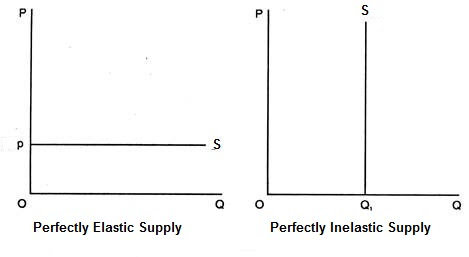
\includegraphics[width=7cm]{perfect elasticities supply.png}
        \end{figure}
    \end{itemize}
\end{frame}

\begin{frame}{Graphical Interpretation of PES (cont.)}
    \begin{figure}
        \centering
        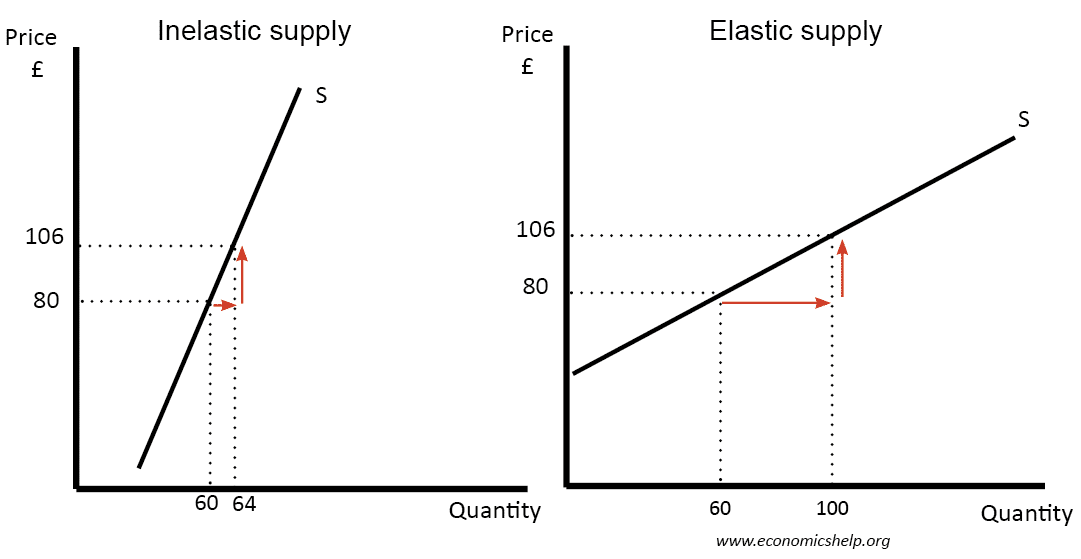
\includegraphics[width=8cm]{elastic-inelastic-supply.png}
        \caption*{Just as before, the rule of thumb and common phrasing is that flatter curves are generally more elastic, and steep curves are generally more inelastic. However, again, this is not technically correct, as supply curves can vary in elasticity based on different factors\footnote{If you want to know more about this, talk to me.}}
    \end{figure}
\end{frame}

\begin{frame}{Graphical Interpretation of PES (cont.)}
    \begin{figure}
        \centering
        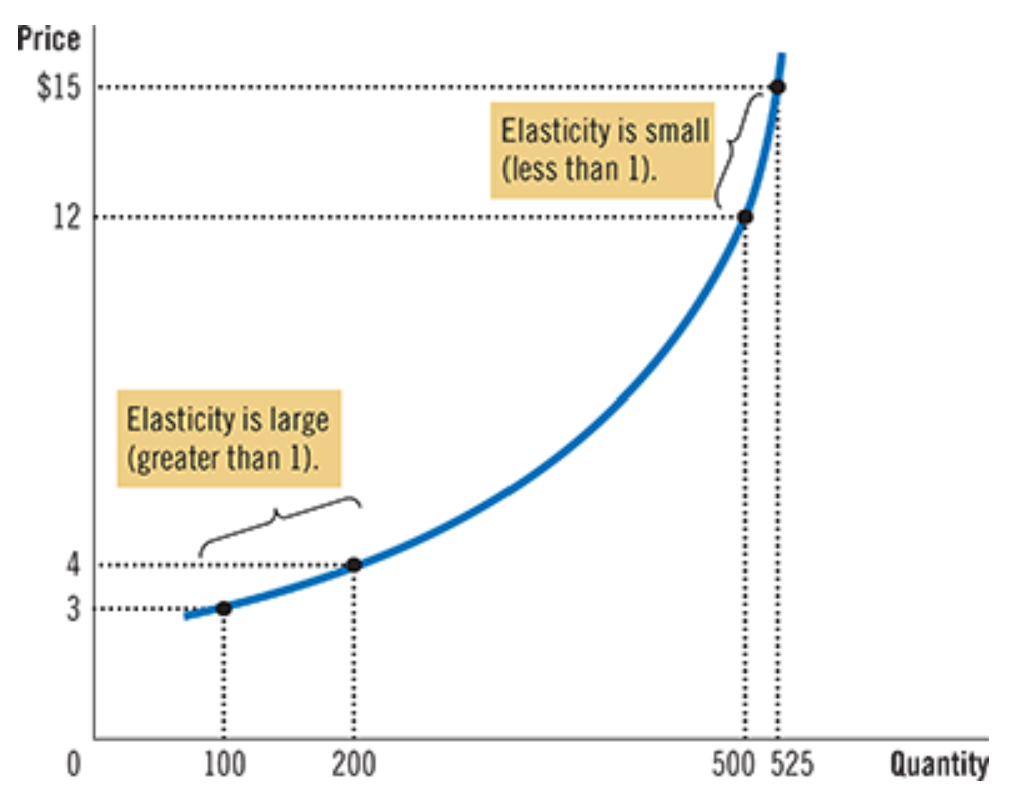
\includegraphics[width=8cm]{curved elastic supply.png}
        \caption*{Flatter portions of a curved supply curve tend to be more elastic, while steeper portions tend to be more elastic}
    \end{figure}
\end{frame}

\begin{frame}{Exercise 3}
    \begin{itemize}[<+->]
        \item In the following diagram, suppose the $Q_{s}$ at $B$ is 14, and $P$ at $A$ is \$600. Find $\epsilon_{S}$
        \begin{figure}
            \centering
            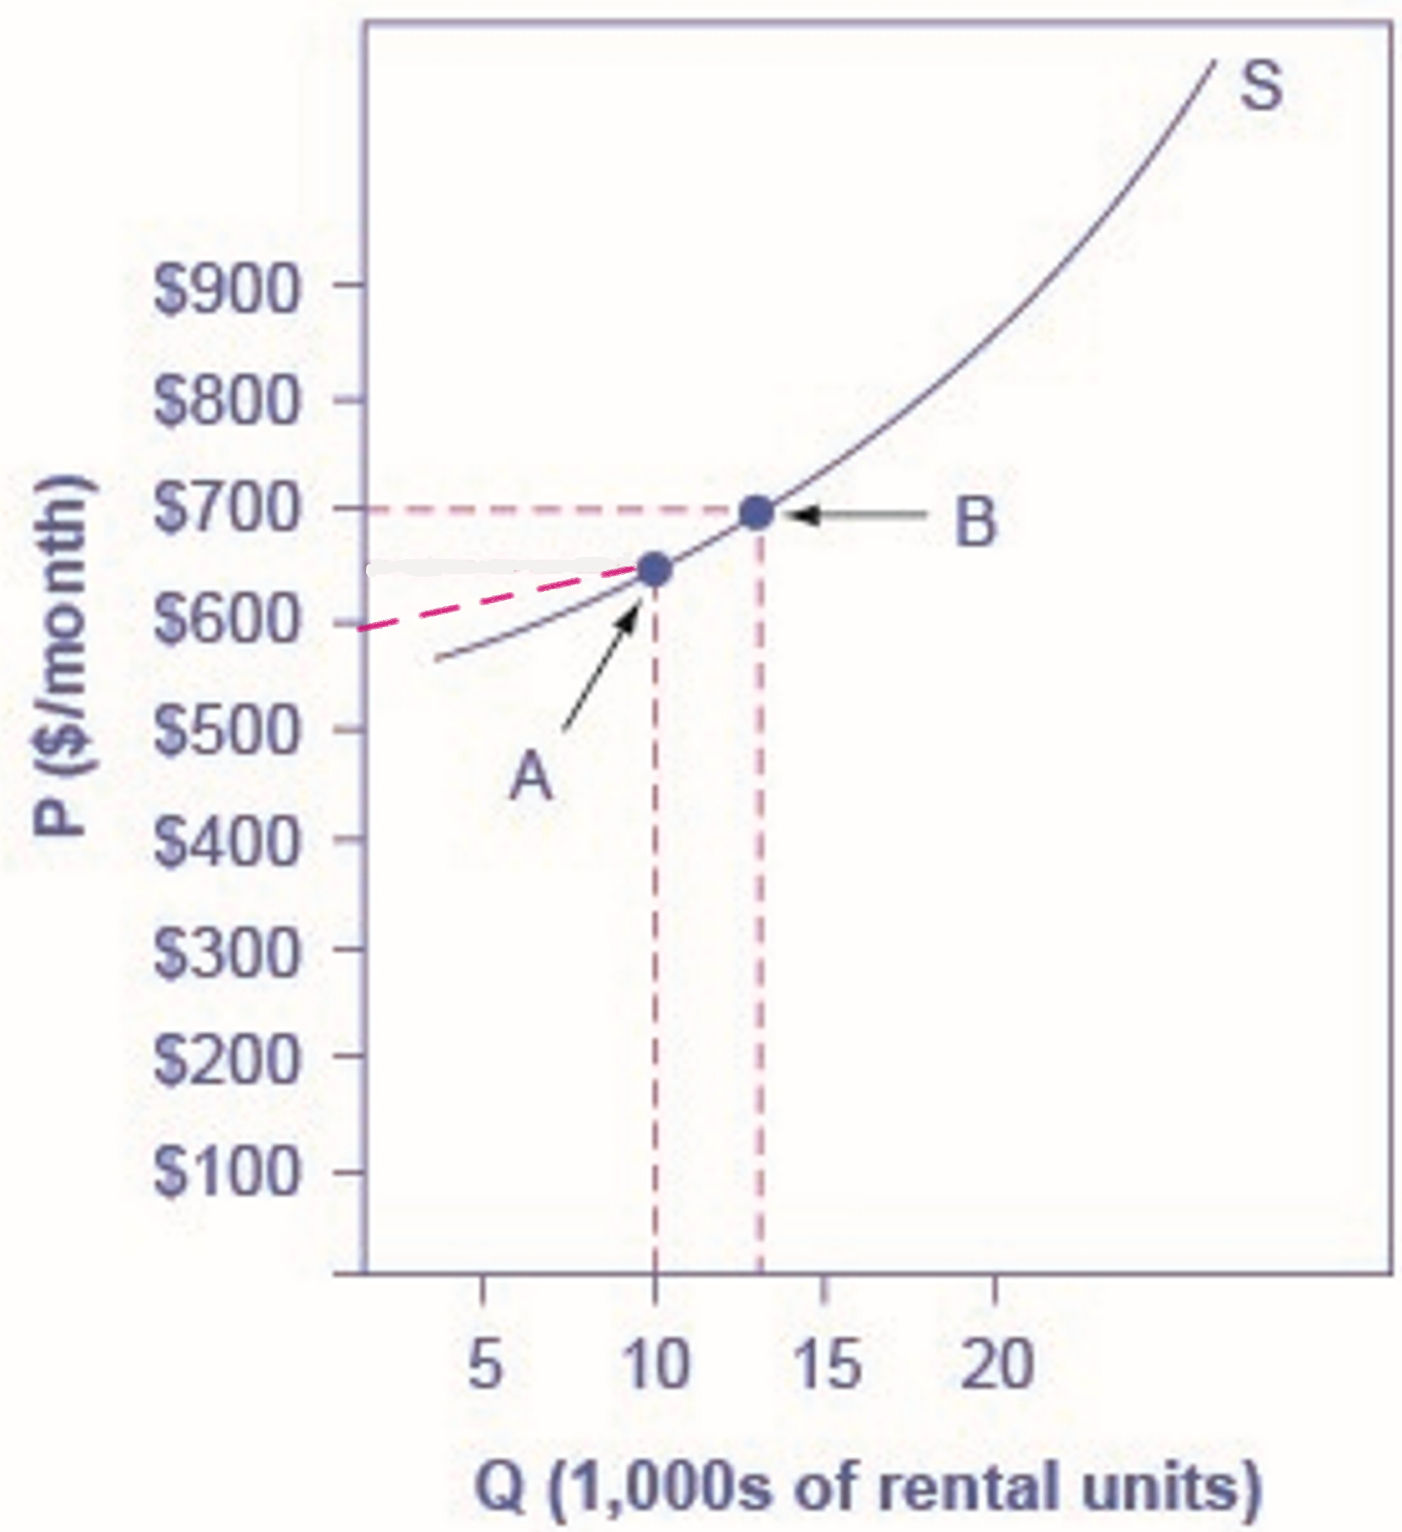
\includegraphics[width=5cm]{supply double example ann.png}
        \end{figure}
    \end{itemize}
\end{frame}

\begin{frame}{Remark about Scaling Units}
    \begin{itemize}
        \item Recall this way of writing the elasticity of supply formula:
        $$\epsilon_{S}=\frac{Q_{2}-Q_{1}}{P_{2}-P_{1}}\cdot \frac{P_{1}+P_{2}}{Q_{1}+Q_{2}}$$
        \item Now, multiplying $Q_{2}$ and $Q_{1}$ by 10 means we get
        \begin{align*}
            \frac{10Q_{2}-10Q_{1}}{P_{2}-P_{1}}\cdot \frac{P_{1}+P_{2}}{10Q_{1}+10Q_{2}}&=\frac{10(Q_{2}-Q_{1})}{P_{2}-P_{1}}\cdot \frac{P_{1}+P_{2}}{10(Q_{1}+Q_{2})}\\
            &=\frac{Q_{2}-Q_{1}}{P_{2}-P_{1}}\cdot \frac{P_{1}+P_{2}}{Q_{1}+Q_{2}}=\epsilon_{S}
        \end{align*}
        \item So the scale of units don't matter when we are doing elasticity change!
    \end{itemize}
\end{frame}

\begin{frame}{Solution 3}
    \begin{itemize}[<+->]
        \item Using the standard $\frac{\Delta Q/[(Q_{1}+Q_{2})/2]}{\Delta P/[(P_{1}+P_{2})/2]}$
        $$\epsilon_{S}=\frac{(14-10)/12}{(700-600)/650}=\frac{13}{6}=2.1\bar{6}$$
    \end{itemize}
\end{frame}

\begin{frame}{Bonus exercise}
    \begin{itemize}[<+->]
        \item Suppose the following curve displays an elasticity of supply equal to 1.69, between points $A$ and $B$. Find the equilibrium quantity after the movement to $B$. Continue to assume $P$ at $A$ is \$600.
        \begin{figure}
            \centering
            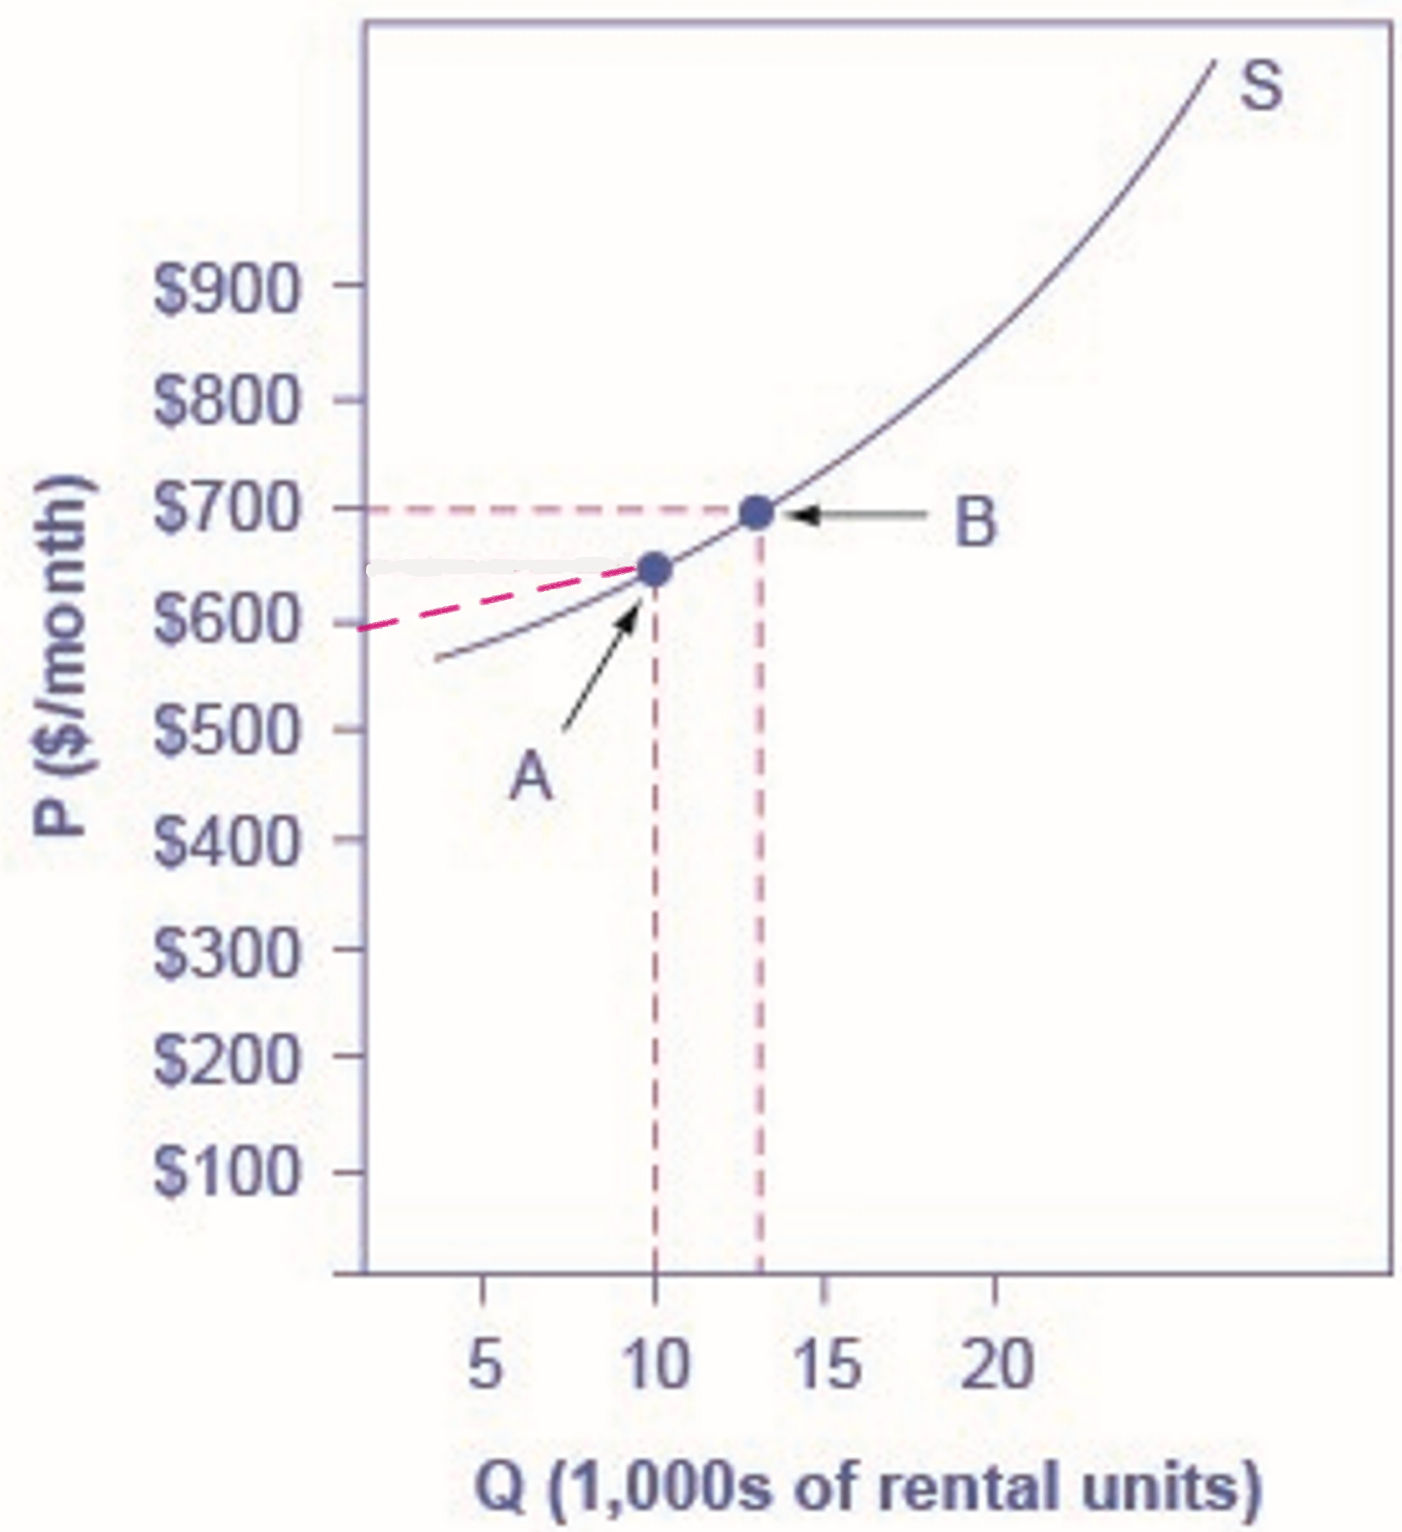
\includegraphics[width=5cm]{supply double example ann.png}
        \end{figure}
    \end{itemize}
\end{frame}

\begin{frame}{Bonus Solution}
    \begin{align*}
        \epsilon_{S}=1.69&=\frac{(Q_{2}-10)/(Q_{2}+10)}{100/1300}\\
        \implies 0.13&=\frac{Q{2}-10}{Q_{2}+10}\\
        \implies 0.13(Q_{2}+10)&=Q{2}-10\\
        \implies 11.3 &= 0.87Q_{2}\\
        \implies Q_{2}&=12.98
    \end{align*}
    \end{frame}

\begin{frame}{Summary of Elasticity}
    \begin{itemize}[<+->]
        \item We want to quantitatively measure the sensitivity of consumers and producers when other factors in the economy change
        \item The measures of focus we are concerned with in this class are [own-] price elasticity of demand, income elasticity [of demand], price elasticity of demand, and elasticity of supply
        \item These are calculated as the percentage change in quantity demanded or supplied, divided by the percentage change in a market factor
        \item To accurately calculate elasticities, we have to have ceteris paribus, and we cannot accurately isolate a market sensitivity if multiple things are changing at once
        \item To calculate percentage change, we use the midpoint method, which is a measure of calculating percent changes that is symmetric (reversible)
        \item Read 5-3 on your own
    \end{itemize}
\end{frame}

\end{document}